%\documentclass[a4paper,9pt,fleqn,notoc]{diss}
%\renewcommand{\includegraphics}[1][1]{} 
%\begin{document}


%%%%%%%%%%%%%%%%%%%%%%%%%%%%%%%%%%%%
\chapter{Grounded Spatial Language Games}
\label{s:spatial-language-games}
\index{spatial language game}
\begin{figure}
\begin{center}
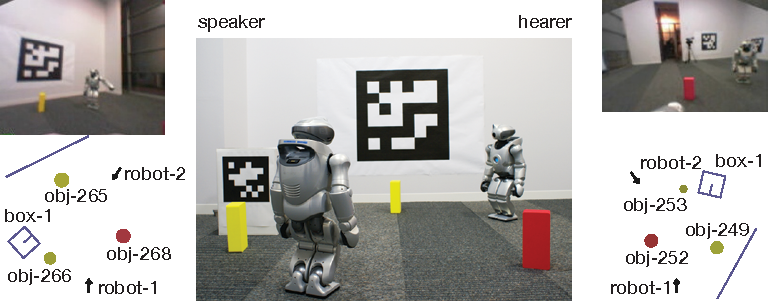
\includegraphics[width=1.0\columnwidth]{figs/space-scene-2-small}
\end{center}
\caption[Example spatial setup]{Example scene. 
Two robots autonomously perceive and act in an office 
environment that contains different types of objects. Both 
robots autonomously create world models reflecting the state 
of the environment (see bottom left and right schematics), that 
include objects with spatial and color properties, the carton boxes 
as well as the robots.}
\label{f:scene}
\end{figure}

Language does not occur in a vacuum. Spoken language occurs in physical,
situated interactions when two interlocutors meet with specific
communicative intentions. This chapter explains the basic social interactions 
at the center of the approach to language. Physical robots meet in communicative
encounters and try to reach communicative goals within real world settings. 
Taking such a radical approach to the study of language is grounded in a number of
social and perceptual mechanisms. Here I look at the prerequisites for 
the computational models discussed later in this book.

Figure \ref{f:scene} shows such an encounter of
two humanoid robots in which one of the robots, the speaker, has the goal
of drawing the attention of the hearer to some object in the environment using language.
Such interactions are called \emph{language game} \citep{steels2001language}\index{Steels, L.}.
Language games are routinized interactions between two members of 
a population. The game combines a particular script for the interaction, the linguistic
information transfer and extra-linguistic feedback about the success of the interaction.
Here is an example of a language game called the \emph{spatial language game}.


\begin{enumerate}
\item The language game starts by randomly drawing two agents from the population. 
One agent is randomly assigned the role of speaker, the other is assigned the role
hearer.
\item The agents establish joint attention and perceive the scene.
\item The speaker chooses an object from the perceived context as the object
he wants to draw the attention of the hearer to.
\item The speaker produces an utterance that he thinks draws the attention to the object.
\item The speaker passes the utterance to the hearer.
\item The hearer interprets the utterance and tries to find the object that the speaker
might have in mind. 
\item The hearer points to the object he thinks the interaction was about. If he was unable 
to interpret a topic, he signals this by shaking his head.
\item The speaker interprets the pointing. If the object pointed to by the hearer
is correct, he signals this by noding. If the hearer pointed to the wrong object or
did not point at all, the speaker
points to the topic he wanted to draw the attention to.
\end{enumerate}


\begin{figure}
\begin{center}
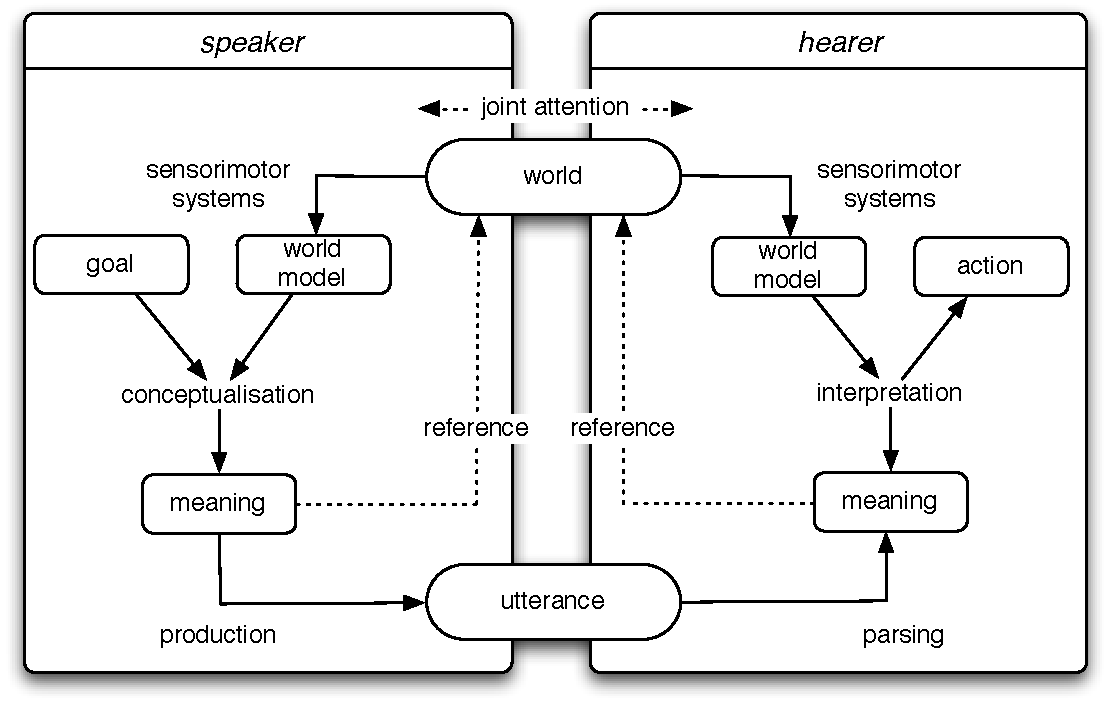
\includegraphics[width=0.9\columnwidth]{figs/semiotic-cycle}
\caption[Semiotic cycle]{\index{semiotic cycle}The semiotic cycle is a model of situated communicative interactions between 
two interacting agents.}
\end{center}
\label{f:semiotic-cycle}
\end{figure}

To study language in a real world  setting requires to fully spell out 
all components involved in the interaction.
Besides social mechanisms agents need operational systems for perceiving
the world, as well as the construction and interpretation of utterances. 
Figure \ref{f:semiotic-cycle} shows a schematic view of the systems
involved in production and parsing, conceptualization and interpretation. 
Both agents independently process sensorimotor data stemming from
the onboard cameras and proprioceptive sensors in order to construct 
world models\index{world model} of the environment 
\citep{spranger2008grounded,spranger2012perception}\index{Spranger, M.}. 
Based on the particular communicative goal and the current state of the 
world represented in the world model, the speaker conceptualizes a meaning 
which is then rendered into an utterance by the language system. 
The hearer parses the utterance to determine its meaning and 
interprets it with respect to his current model of the world in order 
to infer the speaker's communicative goal and, for instance, 
perform a desired action. The system used for conceptualization
and interpretation are explained in detail in Chaper \ref{s:irl}.
The system for producing and parsing utterances is treated in
Chapter \ref{s:fcg}. 
The following sections focus on the necessary prerequisites for 
language production, parsing and evolution in terms of social mechanisms and 
perceptual processing.

\section{Perception}\index{perception}
\label{s:perception}
The environment that robots interact in is equipped with four kinds of objects
that were carefully chosen to pick out special features relevant for spatial language:
\emph{blocks}, \emph{boxes}, \emph{wall markers} and the \emph{robots} themselves 
(see Figure \ref{f:scene}). 
\begin{description}
\item[Blocks] Are the colored brick like objects. They are typically of the same color.
Agents perceive these objects as having a certain distance from their 
egocentric coordinate systems originating in the robot's body.
\item[Boxes] The environment also features card boxes which have 
particular markers on their sides. These markers are perceived by the sensorimotor 
systems as distinct sides of the object. The perceptual systems
perceive them as having a particular distance and orientation with
respect to the robot's coordinate system. 
\item[Wall markers] Figure \ref{f:scene} shows that the same markers
used for the carton boxes can also occur on the wall.
Cardboard boxes introduce a geocentric orientation on the scene.
\item[Robots] Robots also establish the position of the interlocutor in
each interaction. Every robot tracks the position and orientation of the
other robot in his environment.
\end{description}


Before a language game starts the robots perceive their
environment. The robots are endowed with perceptual systems 
for recognizing and tracking the objects in their environment.
These systems continuously build up \emph{world models} of the environment
consisting of sets of objects. The objects are characterized by continuous
real-valued features such as color, position and orientation but also
width, height and length. The perceptual system also provides a basic
grouping of objects into classes such as robots, blocks and boxes and wall markers. 
The following is the world model built by the agent to the left in Figure
\ref{f:scene}. It includes the other robot ({\footnotesize\texttt{robot-2}}), the
landmark ({\footnotesize\texttt{box-1}}) and the colored blocks ({\footnotesize\texttt{obj-265}},
{\footnotesize\texttt{obj-266}} and {\footnotesize\texttt{obj-268}}):
\label{world-model-example}
\begin{footnotesize}
\begin{verbatim}
((robot-1 :type robot :x 0.0 :y 0.0 :orientation 0.5)
 (robot-2 :type robot :x 1461.65 :y -351.24 :orientation 0.9)
 (box-1 :type box :x 513.0 :y 891.67 :orientation 0.36 
        :width 320.0 :height 450.0 :length 310.0)
 (obj-265 :x 1454.74 :y 248.72 :z 0.0 :width 59.75 
          :height 235.99 
          :average-y 128.0 :stdev-y 26.49 :min-y 51.0 
          :max-y 199.0 :average-u ...)
 (obj-266 :x 285.0 :y 549.02 :z 0.0 ...)
 (obj-268 ...)
 (box-wall :orientation 0.36))
\end{verbatim}
\end{footnotesize}


Each robot constructs perceptual representations of the objects in its
immediate surroundings from the raw sensations streaming from the
robot's sensor. Each type of object in the environment is tracked
by a dedicated perceptual system. In general, processing of 
the different object classes is  a three step process.
First, low-level vision routines process raw camera
images to yield basic \emph{percepts} -- these are connected regions that
differ from the background of the environment or are related to 
the patterns distributed on the boxes and wall markers.
Second, these regions are tracked in subsequent
camera images. In order to do so, the vision system needs to establish a
correspondence between an internal \emph{model} and the image
regions that refer to the same physical object, a process known in
robotics as \emph{anchoring} \citep{coradeschi2003anchoring}\index{Saffiotti, A.}\index{Coradeschi, S.}. 
I use state estimation techniques from robotics, e.g. \emph{Kalman Filters} 
\citep{kalman1960linear}\index{Kalman, R. E.}, 
for maintaining such persistent models. Third, the vision system 
fuses information from the proprioceptive sensors of the robot
the visual information to encode a set of visual properties about each object. 
In this particular setup these properties are the position and orientation of objects, 
an estimated width and height and color information. In the experiments 
discussed in this book only position and orientation are relevant. 
Most importantly, the perceptual systems only track objects on the ground. 
The position and orientation of objects is encoded in 
a two dimensional \emph{egocentric} coordinate system which has 
its origin between the two feet of the robot facing to the front of the 
robot. \cite{spranger2008grounded}\index{Spranger, M.} gives more detail on the 
perceptual systems.

The experiments reported on in later sections require that agents play many
language games. In order to speed up the process of a game and in order to
do repeatable, manipulatable experiments, data from spatial scenes\index{spatial scenes}  such as the one 
in Figure \ref{f:scene} are recorded and stored. The output of the perception
system of more than 800 spatial scenes with different spatial configurations 
has been collected and can be accessed by artificial software agents without 
the agents required to run on physical robots.
A spatial language game can be enacted on such stored scenes as if robots 
were perceiving the scene at the very moment they are playing a particular 
language game.

Figure \ref{f:spatial-scenes-1} shows different spatial scenes. Each spatial scene 
consists of a world model for each of the two robots recorded from the position of 
each robot. Scenes are grouped into data sets with similar characteristics
with respect to perspective on the scene, the number of objects and
the availability of boxes and wall markers. For instance, in some data sets the perspective of interlocutors is similar (see Figure \ref{f:spatial-scenes-1} for 
examples from one data set), i.e., robots
are looking at the scene from the same position and there are few objects.
Figure \ref{f:spatial-scenes-2} shows examples from different data sets.

\begin{figure}
\begin{center}
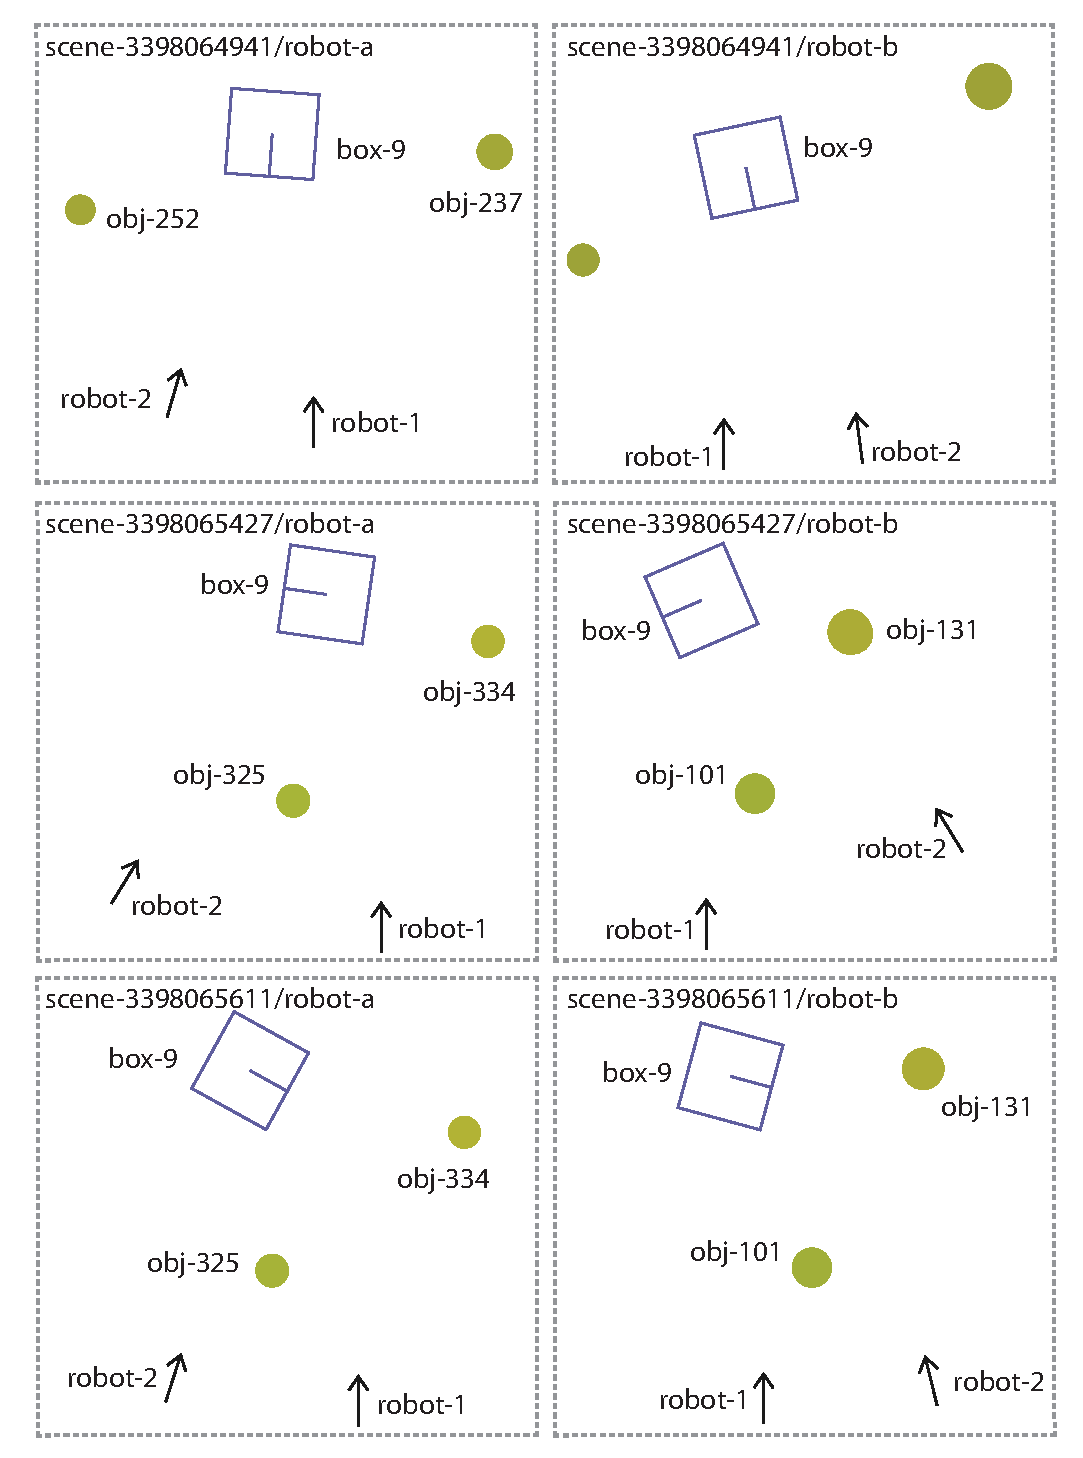
\includegraphics[width=0.8\columnwidth]{figs/spatial-scenes-overview-1}
\end{center}
\caption[Example world models]{Example world models from a spatial data
set called \emph{space-game-2}. Left the world model of 
robot \emph{a} is shown. To the right the world model of robot 
\emph{b} is shown. All scenes share similar properties. In 
this data set robots share a similar perspective on the scene.
The actual position of the robots varies across different scenes, but is always similar.
Similarly, every scene has a box landmark and two yellow blocks in it. 
However, the actual position of the box and its orientation, as well as the
position of the objects change in every scene.}
\label{f:spatial-scenes-1}
\end{figure}

\begin{figure}
\begin{center}
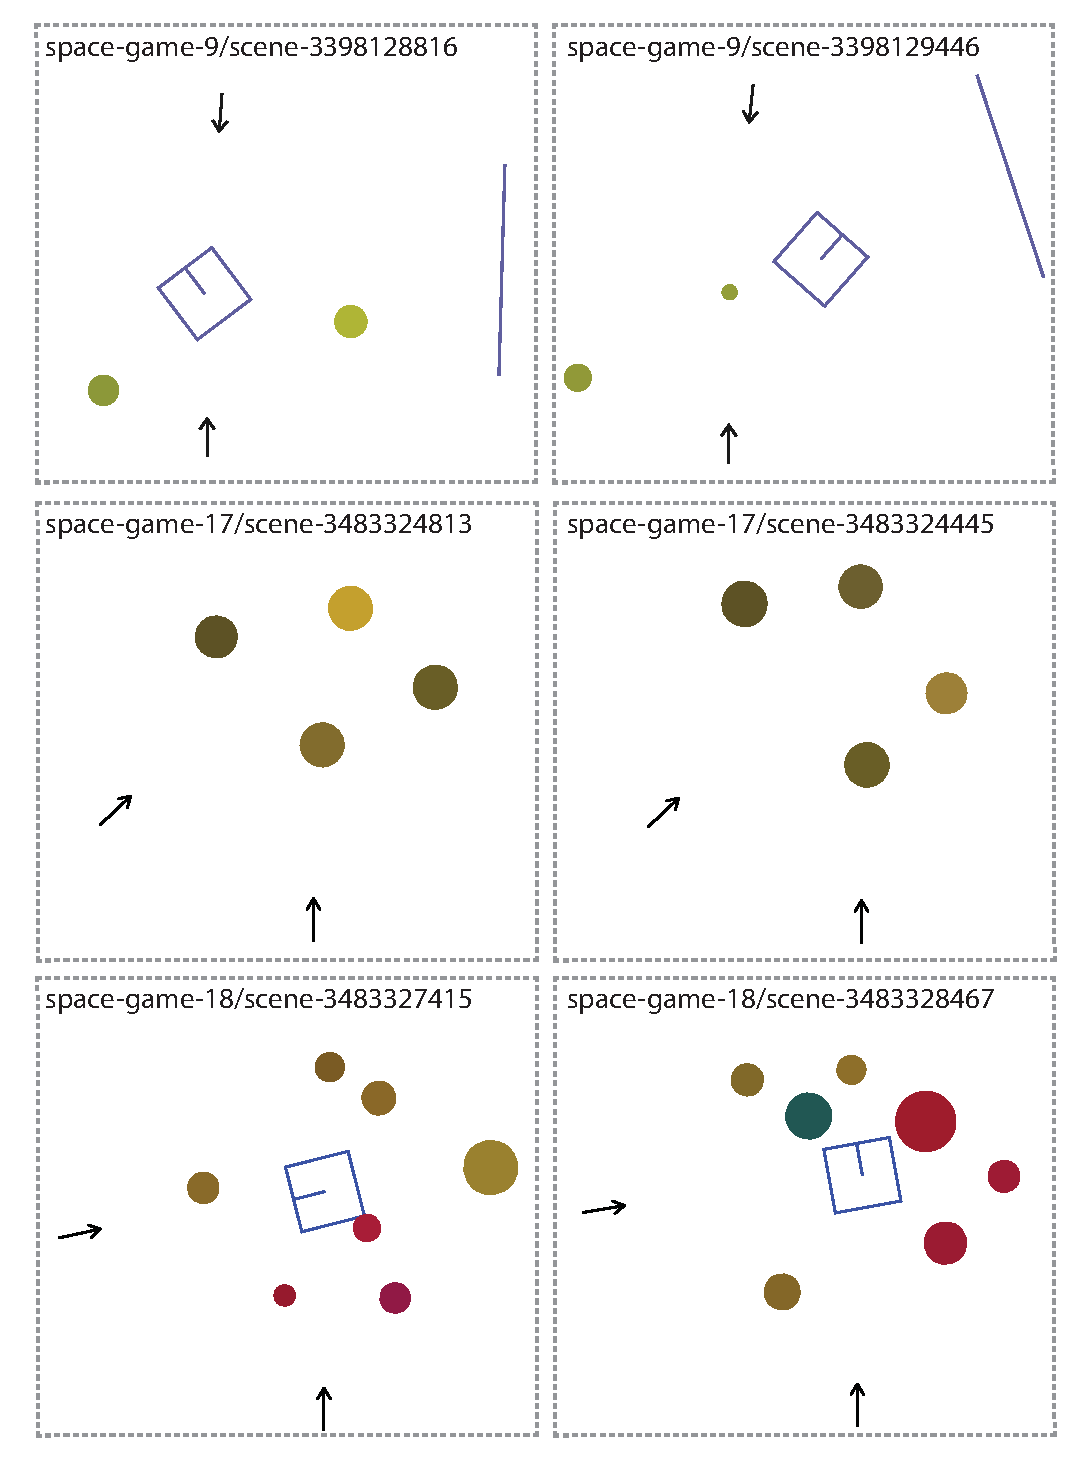
\includegraphics[width=0.8\columnwidth]{figs/spatial-scenes-overview-2}
\end{center}
\caption[Example scenes]{Example scenes from different 
spatial data sets. Each row shows 
scenes from a particular data set (the world model of 
robot \emph{a} is always shown). 
The first row shows a data set which features a global landmark 
(\emph{space-game-9}).
The middle row shows scenes of a data set without global landmark and
without box (\emph{space-game-17}). Lastly, a data set which features 
many objects is shown (\emph{space-game-18}).}
\label{f:spatial-scenes-2}
\end{figure}

\section{Social Mechanisms}
\label{s:social-mechanisms}\index{social mechanisms}
Language games require a number of social mechanisms to be in place. Joint attention, 
turn-taking behavior, pointing and other non-linguistic feedback these are mechanisms 
at the heart of the social interaction. Crucial social mechanisms required for these interaction 
are  considered prerequisites for studying the evolution of language. They constitute the 
background against which communication and evolution of communication takes place.

% joint attention
Joint attentional scenes \citep{tomasello1995joint}\index{Tomasello, M.} in which interlocutors 
are jointly attending to some object for some reasonable amount of time.
Establishing joint attention means in robotic experiments that two robots 
taking part in a language game must (1) share a physical environment, 
(2) attend to a set of objects in their surrounding, (3) track whether the 
respective other robot is able to attend to the same set of objects and 
(4) be able to manipulate attention by pointing to distal objects and perceiving
these pointing gestures  Joint attention is monitored by an external computer 
program, that has access to the world models of both interacting robots.  This system
initiates the interaction between two agents as soon as both agents
observe the same set of objects.  Spatial scenes are manipulated 
by a human experimenter to find spatial setups in which joint attention is
possible, the program monitors whether robots are seeing the same
set of objects and informs the experimenter whether the robots jointly attend 
to the same set of objects.

% turn taking
Social interactions have to be structured, so that agents can interpret the 
signals they exchange. For instance, if the hearer points before
he has received the utterance the speaker will have a hard time 
understanding the gesture. However, if the hearer points after
receiving the utterance, the speaker can assume that this is the response
to his speech act. Language games are coordinated by behavioral scripts. 
Every agent in the population knows the language game script and individually reacts
to changes in the environment and actions of the other robot. For
example the speaker triggers the action of pointing to the intended
topic when the hearer signals that he did not understand the
utterance. The scripts are implemented in the form of finite-state
machines: actions are performed depending on the current state in the
game flow, the perception of the environment and the history of the
interaction.

% non-linguistic feedback
In order to be able to learn and form spatial language systems, 
robots need non-linguistic means of conveying information, such as 
pointing to an object or conveying notions of success, failure and 
agreement in communication.  For demonstration purposes robots are
equipped with pointing gestures but in the communicative interactions 
underlying the results presented in this book, robots use a different 
mechanism in order to avoid further difficulties stemming from uncertainties in pointing (see
\citealp{steels1998stochasticity}\index{Steels, L.}\index{Kaplan, F.} for a discussion of the impact of
such uncertainties on the performance in language games). When a
robot wants to point to an object in the environment, he directly
transmits the coordinates of the intended object to the
interlocutor.  Since robots model object positions in their own
(egocentric) coordinate systems, additional steps have to be taken to
interpret these coordinates.  Most importantly the robot has to know
the position and orientation of the robot that is
pointing.  With this information robots transform the 
coordinates into their own coordinate system and interpret 
the pointing by choosing the closest object to the pointing 
coordinates in their world model. Similarly, robots directly exchange 
other non-linguistic feedback, for instance agreement and 
disagreement in communication by exchanging signals whose
meaning is shared. Moreover, linguistic utterances are directly passed between
interlocutors.



%
%\bibliographystyle{diss}
%\bibliography{papers,space}
%\end{document}

